\subsection{Player}
Klassen "Player" holder styr på spillernes tildelte farve, deres navn, nuværende position, deres forige position, om de er i fængsel og har de et chancekort, som kan få dem ud af fængslet. Dette er klaret på en række af metoder.

Vi har en metode "Player", som gør det muligt for spilleren at skrive et navn, få en farve, få tildelt en "account" og hvilken tur spilleren er på. Dette kan ses på følgende billede:
\begin{figure}[H]
    \centering
    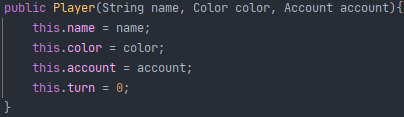
\includegraphics[width=0.7\textwidth]{sources/7_implementering/Player.PNG}
    \caption{Player konstruktør}
    \label{fig:PlayerKonstruktør}
\end{figure}
For at spilleren kan rykke rundt på spillepladen, så har vi lavet matoden "move". Inden spilleren rykker til den nye position, så bliver den tidligere position sat til den nuværende. Derefter lægges spillerens nuværende position sammen med det antal øjne der er slået med terningerne. Hvis man slår nok til, at passere startfeltet, så har vi anvendt modulus, så man kan rykke hele vejen rundt:
\begin{figure}[H]
    \centering
    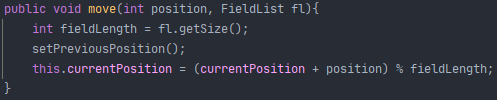
\includegraphics[width=0.7\textwidth]{sources/7_implementering/Move.PNG}
    \caption{Metoder der flytter spilleren}
    \label{fig:PlayerMove}
\end{figure}
Når spillerens tur er overstået, så stiger spillerens "runde-tal" med 1:
\begin{figure}[H]
    \centering
    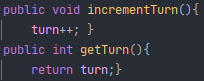
\includegraphics[width=0.7\textwidth]{sources/7_implementering/Turn.PNG}
    \caption{Metode der holder styr på turen}
    \label{fig:TurnKeeper}
\end{figure}
Derefter har vi en række getters \& setters, som holder styr på farve, navn, konto, om spilleren er i fængsel og kan spilleren komme ud af fængsel:
\begin{figure}[H]
    \centering
    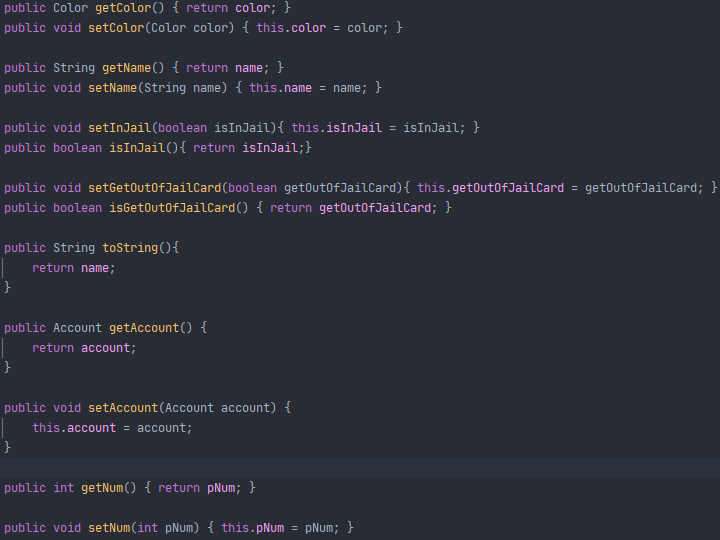
\includegraphics[width=0.7\textwidth]{sources/7_implementering/getSet.PNG}
    \caption{Getters og setters i player klassen}
    \label{fig:GetterSetter}
\end{figure}
